\chapter{Experimentos Preliminares}
\label{chapter:chapter04}

For the initial experimentation phase, there were three different steps taken. First some of the objective functions were tested alone to test if they achieve our required needs. Then is described how the synthetic dataset was created. And finally some initial experiments regarding the comparison between algorithms took place, this with the intention to have as a first approach to test the objective functions and operators, as well as the dataset defined by the previous experiments.

\section{Experiments regarding objective functions}

Some of the objective functions used for the research had a very straightforward approach, the standard deviation $\sigma$ can represent clearly how much variation of different experience levels is inside a a group, and for the group size function, a substraction is the representation of the distance to the ideal group size.\\ 

However the objective functions for the distance between interests and the participation style a representative objective function could not be defined arbitrarely. Therefore, before choosing some experimentation took place, this is described in the following subsections.\\

\subsection{Interests distance function}

For these experiments, four different students were randomly generated with their respective interest set $I_i$, as it was described in Chapter~\ref{chapter:chapter02}. The purpose is to find the distance between $I_1$ and $I_2$. Ideally we want a to have a metric that is a continuous value between 0 to 1, so it doesn't need noramilzation. Several similarity metrics found in \cite{SeyedShirkhorshidi2015AData} and \cite{Sung-HyukChaComprehensiveFunctions} were tested. Then the metrics that didn't give a value a value from 0 to 1 were discarded. This is because when there no common interests between the students in some of the metrics lead to a division by zero. In the end it was established to compare just 2 metrics, these were Cosine Distance $CD$ and Pearson correlation coefficient.\\

The results of this experiment can be seen in Figure~\ref{table:results_interests_comp}, using the sets of interests specified in \ref{table:sample_interests} in the same way it was specified in \chapter{chapter:chapter03}.\\

\begin{table}[]
    \begin{tabular}{llllllllllllllllllllll}
       & Interests    & Business & Property & Enterteinment & Games & Gambling & Films & Animated Films & Family & Dating & Marriage & Fitness & Running & Pets & Hobbies      & Dogs & Travel & Beaches & Arts & Guitar & Dance \\
    $S_1$ & 0.3333333333 & 0.5      & 1        & 0.3333333333  & 0.5   & 1        & 0.5   & 1              & 0      & 0      & 0        & 0       & 0       & 0    & 0            & 0    & 0      & 0       & 0    & 0      & 0     \\
    $S_2$ & 0.3333333333 & 0        & 0        & 0             & 0     & 0        & 0     & 0              & 0.5    & 1      & 0        & 0.5     & 1       & 0.5  & 0.3333333333 & 1    & 0      & 0       & 0    & 0      & 0     \\
    $S_3$ & 0.25         & 0        & 0        & 0             & 0     & 0        & 0     & 0              & 0      & 0      & 0        & 0       & 0       & 0    & 0.3333333333 & 0    & 0.5    & 1       & 0.5  & 1      & 1     \\
    $S_4$ & 0.3333333333 & 0        & 0        & 0.5           & 0     & 0        & 1     & 0              & 0.25   & 0      & 1        & 0       & 0       & 1    & 0.5          & 0    & 0      & 0       & 0    & 0      & 0    
    \end{tabular}
    \caption{Sample interests by student}
    \label{table:sample_interests}
\end{table}

\begin{columns}
    \begin{column}{0.5\textwidth}
        \begin{table}[]
            \begin{tabular}{ll}
            Metric            & Value         \\
            Cosine Similarity & 0             \\
            Pearson + 1       & 0.5662712739  \\
            Pearson           & -0.4337287261 \\
            CD - Pearson      & 0.4337287261 
            \end{tabular}
            \caption{Comparison between $S_1$ and $S_2$}
        \end{table}\\
        \begin{table}[]
            \begin{tabular}{ll}
            Metric            & Value         \\
            Cosine Similarity & 0.02975643611 \\
            Pearson + 1       & 0.6510457773  \\
            Pearson           & -0.3489542227 \\
            CD - Pearson      & 0.3787106588
            \end{tabular}
            \caption{Comparison between $S_2$ and $S_3$}
        \end{table}\\
        \begin{table}[]
            \begin{tabular}{ll}
            Metric            & Value         \\
            Cosine Similarity & 0.04646766902 \\
            Pearson + 1       & 0.7170945873  \\
            Pearson           & -0.2829054127 \\
            CD - Pearson      & 0.3293730817
            \end{tabular}
            \caption{Comparison between $S_3$ and $S_4$}
        \end{table}
    \end{column}
    \begin{column}{0.5\textwidth}
        \begin{table}[]
            \begin{tabular}{ll}
            Metric            & Value         \\
            Cosine Similarity & 0             \\
            Pearson + 1       & 0.6096268784  \\
            Pearson           & -0.3903731216 \\
            CD - Pearson      & 0.3903731216
            \end{tabular}
            \caption{Comparison between $S_1$ and $S_3$}
        \end{table}\\
        \begin{table}[]
            \begin{tabular}{ll}
            Metric            & Value         \\
            Cosine Similarity & 0.2134561996  \\
            Pearson + 1       & 0.9120319917  \\
            Pearson           & -0.08796800825 \\
            CD - Pearson      & 0.3014242079
            \end{tabular}
            \caption{Comparison between $S_2$ and $S_4$}
        \end{table}\\
        \begin{table}[]
            \begin{tabular}{ll}
            Metric            & Value         \\
            Cosine Similarity & 0.1797525892  \\
            Pearson + 1       & 0.8653233148  \\
            Pearson           & -0.1346766852 \\
            CD - Pearson      & 0.3144292744
            \end{tabular}
            \caption{Comparison between $S_1$ and $S_4$}
        \end{table}
    \end{column}
    \caption{Comparison between the sample students}
    \label{table:results_interests_comp}
\end{columns}

\subsection{Participation style Function}

The purpose for the participation style function is to reduce the \textit{quantity of silence} in the conversations of a group to a minimum. Therefore The objective function should have a relationship between this \textit{quantity of silence}. In the literature there isn't already a metric or a mathematical function that is able to tell how much silence will be produced in a determined conversation. What has been found is a model created by Benne and Sheats \cite{FunctionalRoles} that assigns a \textit~{Functional Role} label to the intention each of the utterances have in a conversation. It is easy to assume that there must be a correlation between the \textit{quantity of silences} in a conversation and the \textit{Functional Role} or a combination of \textit{FunctionalRoles} in a conversation.\\

To understand the behaviour in a conversation it was proposed to make a brief data analysis of a group of conversation and check the interaction between the silence quantity and the functional roles. For this analysis it was found a well-known dataset AMI meeting corpus \cite{mccowan2005ami} which has previously been used in other works like \cite{dong2012modeling} and \cite{Matsuyama2015Four-participantParticipant}. The dataset includes several conversations of different meetings with different people, with markers of time indicating when each utterance occur, along with some notes and a accompanying video. Some of the meetings found in this dataset had also been labeled with their correspondent Functional role for each utterance by \cite{dong2012modeling}.\\

The meetings used for these analysis have the following names: "ES2002d", "ES2008b", "ES2008d", "ES2009d" and "IS1003d". The first task was to analyze the \textit{quantity of silences} and their duration. Fortunately each utterance also has a start time and and end time, so the proportion of the conversation which was silence is considered as the time in which no utterance is occurring. For each meeting, the total silence time in seconds was considered as the proportion corresponding to the total conversation time, the results can be seen in Table~\ref{table:ami_times}.\\

\begin{table}[]
    \label{table:ami_times}
    \begin{tabular}{lll}
            & Total Silence time & Silence proportion \\
            ES2002d & $6861.49s$         & $72.89\%$  \\
            ES2008b & $7867.38s$         & $75.24\%$  \\         
            ES2008d & $6973.49s$         & $78.23\%$  \\         
            ES2009d & $5963.49s$         & $70.49\%$  \\         
            IS1003d & $5514.33s$         & $66.78\%$          
    \end{tabular}
\end{table}

One of the conversation functional roles of Benne and Sheats is descibed as "protagonism". This infers that a person making an utterance with this intention is starting to talk about a specific topic, not just responding by the utterance made by others. It was infered that this specific role may have some correlation with the lack of silences. The next step involved measuring the \textit{protagonistic proportion} and \textit{protagonistic time} of each of the participants in the conversation. This is for all the utterance they made, how many were \textit{protagonistic} and for all the time they spoke, how much of it was \textit{protagonistic} restectively.\\

In Table~\ref{table:res_ES2008d} and Table\ref{table:res_IS1003d} shows the \textit{protagonistic proportion} and \textit{protagonistic time} for each participant in the conversation with the most (ES2008d) and the less (IS1003d) \textit{quantity of silences}. As it can be seen in (ES2008d) is only brief protagonisms by a single person in the conversation, while (IS1003d) has a homogeneus amount of \textit{protagonisms} by all of their participants.\\

\begin{table}[]
    \begin{tabular}{lll}
    Participant & Protagonism proportion & Protagonistic time \\
    A           & $9.46\%$                & $3.97\%$            \\
    B           & $0.58\%$                & $0.23\%$            \\
    C           & $4.19\%$                & $1.86\%$            \\
    D           & $15.9\%$                & $5.16\%$           
    \end{tabular}
    \caption{Protagonism proportion for the Meeting IS1003d}
    \label{table:res_IS1003d}
\end{table}

\begin{table}[]
    \begin{tabular}{lll}
    Participant & Protagonism proportion & Protagonistic time \\
    A           & $9.29\%$               & $3.2\%$            \\
    B           & $0.0\%$                & $0.0\%$            \\
    C           & $0.0\%$                & $0.0\%$            \\
    D           & $0.0\%$                & $0.0\%$           
    \end{tabular}
    \caption{Protagonism proportion for the Meeting ES2008d}
    \label{table:res_ES2008d}
\end{table}

Finally the quantity of participations was compared to the average participation and the summation of these participations, shown in Table~\ref{table:results_ami}. Here we proposed a inverse correlation to the sum of participations $\frac{1}{\sigma}$ as the metric for improving the number of participations and therfore lowering the \textit{quantity of silence}, as it can be seen in Table~\ref{table:results_ami}, a low value of it represents a positive impact in the quantity of participations.\\

\begin{table}[]
    \begin{tabular}{lllll}
    Conversation & Participations proportion & Average  of paticipation & $\Sigma$ & $\frac{1}{\sigma}$ \\
    ES2008b      & $24.75\%$                 & $0.80\%$                                                              & $23.17\%$  & $4.3$               \\
    ES2008d      & $24.16\%$                 & $5.79\%$                                                              & $3.21\%$   & $31.17$              \\
    ES2002d      & $27.11\%$                 & $4.29\%$                                                              & $17.15\%$  & $5.83$               \\
    ES2009d      & $29.51\%$                 & $2.43\%$                                                                & $9.72\%$   & $10.29$              \\
    IS1003d      & $33.21\%$                 & $2.81\%$                                                                & $11.23\%$  & $8.90$             
    \end{tabular}
    \caption{Results of the conversation analysis}
    \label{table:results_ami}
\end{table}

It should be noticed that this, by no means is considered a strong data analysis, nor the objective function should be considered as definitive. But as a first approach and considering the information that could be gathered at the moment it serves its purpose for the sake of this research.\\

\section{Synthetic dataset creation}

In order to calculate the value for each objective function described in the previous Chapter~\ref{chapter:chapter03} is necessary to consider some features about each student regarding their experience level, their interests and their participation style.\\

The experience level is represented as a numerical quantity described in Chapter~\ref{chapter:chapter03}, for the interests it was considered a fixed size of 3 interests for each one of the students, and a feature representing the participation style was considered as the percentage of the Benne and Sheats role \cite{FunctionalRoles} of "Protagonist" that a student has on average in a conversation.\\

Since these features have never been used in any other scenario togheter, there wasn't a specific dataset that included all of them, therefore a Synthetic dataset was created. This dataset was designed in such a way that resembles what a real dataset would look like once there is data gathered for each of the features, this includes using the statistical distributions: mean and the standard deviation for the generation of the synthetic data, In the following subsections is discussed how this data was obtain and other important details for the dataset creation.\\

In the following subsection is described where the metrics (mean and standard deviation) comes from and why were they used.\\

\subsection{Experience Level} 

While there isn't distribution information for the language levels for CEFR specifically, the IELTS has a data about the frequency distributions by percentage \cite{ielts_demographic_data_2018} which has a distribution by a given level, fortunetly these levels have their equivalence in the CEFR scale, these proportion can be seen in Table~\ref{table:results_levels}.\\

\begin{table}[]
    \begin{tabular}{ll}
    CEFR Level & Proportion \\
    A0         & 0.33\%     \\
    A1         & 0.33\%     \\
    A2         & 0.33\%     \\
    B1         & 13.0\%     \\
    B2         & 48.0\%     \\
    C1         & 36.0\%     \\
    C2         & 2.0\%     
    \end{tabular}
    \caption{The distribution by each level}
    \label{table:results_levels}
\end{table}

\subsection{Interests} 

Like it was previously mentioned in \chapter{chapter:chapter02} Facebook has a database of interests distributed across the population by regions. This data corresponds to the ontology presented in \chapter{chapter:chapter02}. The main purpose of the Facebook Ad platform \ref{facebook_business} is to make marketing campagins.\\

When a user of this platform consults the potential marketing segment filtering by a specific interest a number is shown know as \textit{Potential reach}. This number was aquired for each interest in the ontology to figure out the proportion of each interest.\\

It should be noticed that the overall interests categories (such as "Business and Industry" or "Hobbies") weren't considered for this, because they represented very general interest and represented a significant portion of the overall interests. Therefore only interests from the third level in the ontology onward were considere to get this proportion.\\

A portion of the resulting distribution of interests can be seen in Table~\ref{table:results_interests}

\begin{table}[]
    \begin{tabular}{ll}
    Interest name              & Proportion \\
    Television programme       & 62.94\%    \\
    Restaurants                & 45.88\%    \\
    Vehicles                   & 27.25\%    \\
    Sports                     & 13.00\%    \\
    Music                      & 8.21\%     \\
    Arts and music             & 5.29\%     \\
    Travel                     & 5.11\%     \\
    Films                      & 4.61\%     \\
    Reading                    & 4.51\%     \\
    Consumer electronics       & 4.43\%     \\
    Games                      & 4.18\%     \\
    Shopping                   & 3.68\%     \\
    Beauty                     & 3.49\%     \\
    Live events                & 3.21\%     \\
    Politics and social issues & 2.96\%     \\
    Food                       & 2.87\%     \\
    Computers                  & 2.48\%     \\
    Pets                       & 2.29\%     \\
    Clothing                   & 2.07\%     \\
    Drinks                     & 2.04\%    
    \end{tabular}
    \caption{The first 20 Interests and their proportion}
    \label{table:results_interests}
\end{table}

\subsection{Participation style}

For the participation style, the same dataset as for defining the function was used, the AMI meeting corpus. since we established the metric to be used as the \textif{proportion of protagonisms}, the mean and standard deviation were calculated directly per person in each conversation, the results of this can be seen in Table~\ref{table:participation_results}.\\

\begin{table}[]
    \begin{tabular}{ll}
    Protagonism mean               & $9.67$ \\
    Protagonism standard deviation & $6.66$
    \end{tabular}
    \caption{Results for the Participation Analysis}
    \label{table:participation_results}
\end{table}

\section{Exploratory Experiments}

Before comparing all the proposed algorithms, several exploratory experiments took place, with the idea of understanding how the objective functions as well as the proposed operators behave. This also serves as a first comparison of a simple metaheuristic, a population based metaheuristic and a multiobjetive algorithm. 

All algorithms were subject to similar parameters, described as follows.

\begin{itemize}
    \item The dataset $n=10,001$ was used. The mutation operator described in \ref{chapter:chapter03} at a $0.5$ rate.

    \item For the single objective algorithms, the same weight for all the functions was considered.
    
    \item For the population based algorithms $GA$ and $NSGA-II$ the crossover operator defined in \ref{chapter:chapter03} was used at a $0.9$ rate.

    \item Also, for the population based algorithms, a population of $p=40$ was considered. 
    
    \item All the algorithms ran for over $10,000$ evaluations, which means $10,000$ steps for $LS$, and $250$ generations for $GA$ and $NSGA-II$
\end{itemize}

\subsection{Single Objective Optimization}

For the single objective problems a composed function was proposed, seen in Equation~\ref{weighted_function}, considering each of the objective functions previously defined. This also serve as the basis for comparison between these single objective and multi objective experiments.\\

\begin{itemize}
\item Funcion for the group size \(f_{1}\)
\item Function for the interests similarity \(f_{2}\)
\item Function for the similarity of experience level \(f_{3}\)
\item Function for the participation style \(f_{4}\)
\end{itemize}

\begin{equation} \label{weighted_function}
    f = w_{1} \times f_{1} + \\
    w_{2} \times f_{2} + \\
    w_{3} \times f_{3} + \\
    w_{4} \times f_{4}
\end{equation}

\subsubsection{Local Search}

For the first experiment, a $LS$ algorithm was used, since this is considered one of the most simple metaheuristics that can be used for single-objective optimization according to the literature. As it can be seen in Figure~\ref{fig:local_search} from a random solution the algorithm manages to improve until it gets stuck in a local minima.

\begin{figure}
    \centering
    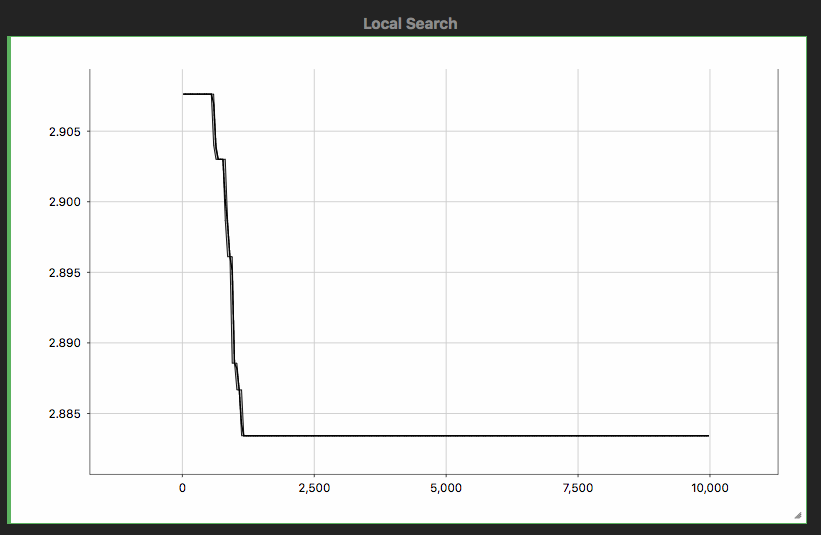
\includegraphics[width=\textwidth]{Local.png}
    \caption{Búsqueda Local}
    \label{fig:local_search}
\end{figure}

\subsubsection{Genetic Algorithm}

$LS$ is a metaheuristic that only makes a single change per step. However it was necessary to also test a population based approach to test the proposed crossover operator. An experiment using a $GA$ was also tested with similar to $LS$. As it can be seen in Figure~\ref{fig:} the algorithm manages to improve for the first $100$ steps until it reaches a local minima, then it continues moving to worse solutions. This algorithm ran for over $250$ iterations using a population of $40$ and a crossover rate of $0.9$. With $0.5$ mutation rate. The largest dataset of $n=10,001$ was used and each of the objective functions having the same weight, just as used by $LS$.

\begin{figure}
    \centering
    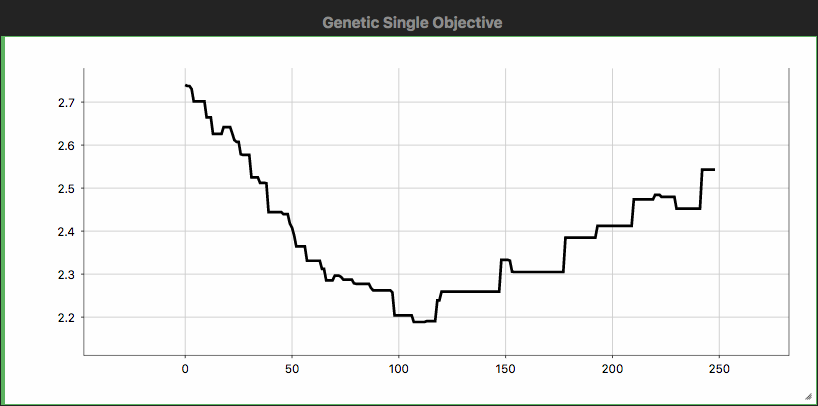
\includegraphics[width=\textwidth]{Genetic.png}
    \caption{Algoritmo Genético Mono-objetivo}
    \label{fig:genetico}
\end{figure}

\subsection{Multi-Objective Algorithm}

For the single objective optimization it was decided to use NSGA-II, since is one of the most common algorithms found in the literature and has mostly the same parameters as the single objective genetic algorithm.

In order to compare it to the single-objective algorithms, the result of each objective function was added between them in each generation step. 
As it can be seen in Figure~\ref{fig:} the algorithm is stuck at several local minima but it manages to continue improving. It also should be noticed that it improves significantly better than its single-objective counterparts.

\begin{figure}
    \centering
    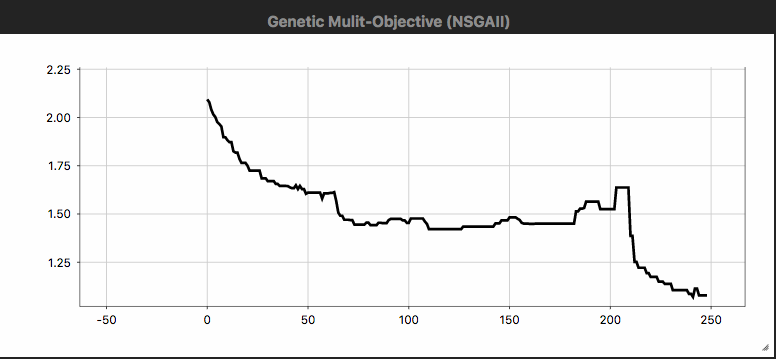
\includegraphics[width=\textwidth]{Multi-Objective.png}
    \caption{Multi-Objetivo (NSGAII)}
    \label{fig:multiobjetivo}
\end{figure}
